\documentclass[a4paper,titlepage,12pt]{article}

%% Language and font encodings
\usepackage[swedish]{babel}
\usepackage[utf8]{inputenc}
\usepackage{textcomp}
\usepackage{amsmath}
\usepackage{graphicx}
\usepackage[colorinlistoftodos]{todonotes}
\usepackage{afterpage}
\usepackage[colorlinks=true, urlcolor=blue, linkcolor=black, pdfborder={0 0 0}]{hyperref}
\usepackage{longtable}
\usepackage[yyyymmdd]{datetime}
\usepackage[bottom]{footmisc}
\usepackage{titling}
\usepackage{pbox}
\usepackage{booktabs}
\usepackage{color, colortbl}
\definecolor{Gray}{gray}{0.9}
\usepackage{changepage, titlesec}

%Set page size
\usepackage{geometry}
\geometry{margin=3cm}
\usepackage{parskip} 
\setcounter{secnumdepth}{5}


\renewcommand{\dateseparator}{-}
\addto\captionsswedish{% Replace "swedish" with the language you use (if using babel)
  \renewcommand{\contentsname}%
    {Innehållsförteckning}%
}

%%%%%%%%%%%%%%%%%%%%%%%%%%%%%%%
% Header and footer
%%%%%%%%%%%%%%%%%%%%%%%%%%%%%%%

\usepackage{fancyhdr}
\pagestyle{fancy}

\lhead{
\includegraphics[scale=0.3]{images/logga.png}}
\chead{System för 3D-kopiering}
\rhead{\today}
\setlength\headheight{26pt} 


\lfoot{TDDD96 --- PUM}
\rfoot{Grupp 9}

\posttitle{\end{center}}

\begin{document}
\begin{titlepage}

% Title text
\topskip0pt
\vspace*{\fill}
\huge
\textbf{Teknisk dokumentation} \\
\Large
System för 3D-kopiering \\
\noindent\rule{17cm}{0.4pt}
\bigskip

\small
\textbf{Hampus Dunström \\
Olof Holmberg \\
Gustav Jannering \\
Michael Karlsson \\
Martin Lundberg \\
Hannes Tuhkala \\
Fredrik Wallström}
\bigskip
\bigskip

Handledare: Sam Le \\
Examinator: Kristian Sandahl

\date{\today}
\vspace*{\fill}

% Image 
\vspace*{\fill}
\begin{minipage}[b]{0.7\textwidth}
	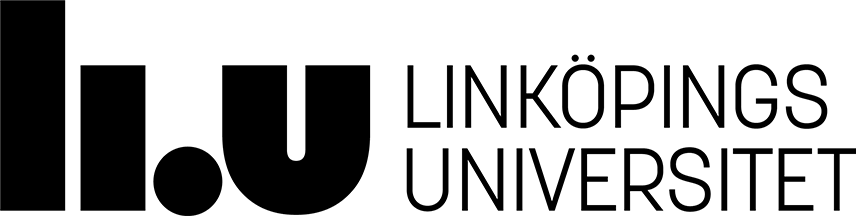
\includegraphics[width=8cm]{images/liu-logga.png}
\end{minipage}
\begin{minipage}[b]{0.4\textwidth}
	\normalsize
	\textit{Linköpings universitet} \\
	\textit{SE-581 83 Linköping, Sverige}\\
	\textit{013-28 10 00, www.liu.se}
\end{minipage}

\end{titlepage}
\newpage
\begin{center}
\pagenumbering{gobble}


%%%%%%%%%%%%%%%%%%%%%%%%%%%%%%%%%%%%%%%%%%%%%%%%%%%%%%%%%%%%%%%%%%%%%
%						Medlemmar
%%%%%%%%%%%%%%%%%%%%%%%%%%%%%%%%%%%%%%%%%%%%%%%%%%%%%%%%%%%%%%%%%%%%%
\section*{\centering Projektidentitet}

System för 3D-kopiering, VT 2017, PUM-9 \\ 
Linköpings Tekniska Högskola, IDA
  
\bigskip

\scalebox{0.8}{
\begin{tabular}{|l|l|l|l|}
	\hline
    \rowcolor{Gray}
	\textbf{Namn} & \textbf{Ansvar} & \textbf{Telefon} & \textbf{E-post} \\
	\hline
    Hampus Dunström & Utvecklingsledare & 0763279292 & hamdu013@student.liu.se\\
    \hline
    Olof Holmberg & Testledare & 0725227007 & oloho254@student.liu.se\\
    \hline
    Gustav Jannering & Analysansvarig & 0706567093 & gusja113@student.liu.se\\
    \hline
    Michael Karlsson & Teamledare & 0735807120 & micka199@student.liu.se\\
    \hline
    Martin Lundberg & Arkitekt & 0762436905 & marlu819@student.liu.se\\
    \hline
    Hannes Tuhkala & Dokumentansvarig \& konfigurationsansvarig & 0760175790 & hantu447@student.liu.se\\
    \hline
    Fredrik Wallström & Kvalitetssamordnare & 0705826972 & frewa814@student.liu.se\\
    \hline
\end{tabular}}

\bigskip
\textbf{Beställare}: Maria Magnusson, maria.magnusson@liu.se 
\\Linköpings universitet ISY

\newpage
\tableofcontents
\newpage

%%%%%%%%%%%%%%%%%%%%%%%%%%%%%%%%%%%%%%%%%%%%%%%%%%%%%%%%%%%%%%%%%%%%%
%					Dokumenthistorik
%%%%%%%%%%%%%%%%%%%%%%%%%%%%%%%%%%%%%%%%%%%%%%%%%%%%%%%%%%%%%%%%%%%%%
  \section*{\centering Dokumenthistorik}
  \renewcommand*{\arraystretch}{1.4}
 \centering
\scalebox{1.1}{
\begin{tabular}{|l|l|l|l|}
	\hline
    	\rowcolor{Gray}
	\textbf{Version} & \textbf{Datum} & \textbf{Utförda förändringar} & \textbf{Utförda av} \\
	\hline
    	1.0 & 2017-06-01 & Första version & Gruppen \\
    	\hline
\end{tabular}}
\end{center}
\newpage

%%%%%%%%%%%%%%%%%%%%%%%%%%%%%%%%%%%%%%%%%%%%%%%%%%%%%%%%%%%%%%%%%%%%%
%					Introduction
%%%%%%%%%%%%%%%%%%%%%%%%%%%%%%%%%%%%%%%%%%%%%%%%%%%%%%%%%%%%%%%%%%%%
\pagenumbering{arabic}
\section{Inledning}
	Detta dokument är en teknisk dokumentation över systemet för 3D-kopieringsprojektet på Linköpings universitet. Projektet pågick under vårterminen 2017 och utfördes av sju stycken studenter ifrån universitetet. Projektet är en del i kursen TDDD96 - Kandidatprojekt i programvaruutveckling som ges vid Linköpings universitet. Den tekniska dokumentationen beskriver hur produkten är utvecklad och hur den fungerar.
	\subsection{Parter}
		Under projektets gång fanns följande parter aktiva:
		
		\begin{itemize}
			\item Beställare \& Kund: Maria Magnusson, Linköpings universitet ISY
			\item Examinator: Kristian Sandahl
			\item Handledare: Sam Le
			\item Projektgrupp: 3DCopy
		\end{itemize}
		
	\subsection{Definitioner}
		Nedan följer definitioner och ordval som används i denna användarmanual.
		
		\begin{itemize}
			\item ISY - Institutionen för systemteknik
			\item ICP - Iterative closest point (iterativ närmast punkt)
			\item PCL - Point cloud library
		\end{itemize}
    
\newpage  

\section{Systemöversikt av 3DCopy}
Systemet består i huvuddel av två stora komponenter: en registreringskomponent och en meshningskomponent. Registreringskomponenten har som syfte att registrera punktmoln så att de bildar en komplett eller fullständig modell av ett punktmoln. Meshningskomponenten har som syfte att generera en 3D-mesh utifrån det kompletta punktmoln som registrerats i registreringskomponenten eller utifrån ett annat komplett punktmoln. Systemet innehåller också ett filter vars syfte är att filtrera olika punktmoln vid behov. Detta för att ta bort onödiga/redundanta punkter. Det finns också ett CLI och ett GUI för att kunna använda själva programmet. 

%%%%%%%%%%%%%%%%%%%%%%%%%%%%%%%%%%%%%%%%%%%%%%%%%%%%%%%%%%%%%%%%%%%%%
%					Systemet
%%%%%%%%%%%%%%%%%%%%%%%%%%%%%%%%%%%%%%%%%%%%%%%%%%%%%%%%%%%%%%%%%%%%%
\section{Systemet/3Dcopy} % Välj namn
	Nedan gås systemet igenom mer ingående.
	
	\subsection{Registreringskomponent}
		Registreringskomponenten är implementerad som en klass i C++. Syftet med registreringen är att generera ett komplett punktmoln utifrån flera icke kompletta punktmoln. Registreringsklassen tar in en vektor med flera icke kompletta punktmoln. Klassen går sedan igenom alla punktmoln i vektorn och registrerar dessa parvis till ett komplett punktmoln. För att uträtta detta används algoritmen ICP ifrån biblioteket PCL. Algoritmens metod för att registrera punktmolnen går ut på att minimera avståndet mellan punkterna i molnen. När sedan ett komplett punktmoln har genererats returneras detta. För registrering finns följande parametrar som kan ändras:
		
		\begin{itemize}
			\item Max Iterations - anger hur många registreringsiterationer som algoritmen får utföra innan den tvingas avsluta.
			\item Transformation Epsilon - avgör hur stor förflyttning algoritmen får göra på målmolnet inom en iteration. 
			
			\item Max Correspondence Distance - anger hur stort avståndet från en punkt i ursprungsmolnet till motsvarande punkt i målmolnet får vara. Är avståndet större än detta kommer algoritmen ignorera punkten i målmolnet vid registreringsförsöket. 
			
			\item RANSAC Outlier Rejection Threshold - anger hur stort avstånd som en punkt tillåts existera från den antagna matematiska modellen för att användas i registreringen. RANSAC, Random Sample Consensus är en metod för att avgöra om en punkt följer det matematiska mönster som algoritmen letar efter.
			
			\item Euclidean Fitness Epsilon - representerar det fel som accepteras. Är skillnaden i felet mellan två iterationer mindre än det här kommer algoritmen avsluta.
			 
		\end{itemize}
	Dessa parametrar kan ändras för att optimera registreringen för specifika punktmoln. 
	
	\subsection{Meshningskomponent}
		Meshningskomponenten är implementerad som en klass i C++. Syftet med meshningen är att generera en 3D-mesh utifrån ett komplett punktmoln. En 3D-mesh är ett 3D-objekt uppbyggt av polygoner. Denna 3D-mesh används för att göra det möjligt att skriva ut objektet i en 3D-skrivare. 
		
		Meshningsklassen tar in ett komplett punkmoln som parameter och tar sedan ut alla punkters normaler i molnet. För att generera en 3D-mesh används Poisson surface reconstruction (PSR) algoritm i PCL. Algoritmen kräver en uppsättning av 3D-punkter med orienterade normaler för att kunna generera en mesh av objektet. Klassen returnerar sedan den färdiga meshen.
		
		Vid meshning av ett objekt kan olika parametrar justeras, beroende på objekt, för att eventuellt förbättra den genererade meshens utseende. De parametrar som kan justeras presenteras nedan.
		
		\begin{itemize}
			\item \textit{depth} - Sätter det maximala djupet i sökträdet som PSR använder sig av, högre värde betyder bättre resultat men blir mer beräkningstungt.
			\item \textit{solver\_divide} - Denna parameter anger vilket djup ett Gauss-Seidel-solver block ska använda för att lösa Laplacian-ekvationen i PSR. Använda denna parameter hjälper att reducera minneskostnaden till en kostnad för rekonstrueringstid.
			\item \textit{samples\_per\_node} - Specificerar det minsta antalet punkter som PSR sätter i en octree-nod då ytan rekonstrueras. Vid brusig punktdata kommer ett högt värde (6-10) jämna ut meshen, men riskerar att tappa detaljer av objektet. Ett lågt värde (1-5) behåller detaljerna men meshen kan bli mer oslipad.
			\item \textit{point\_weight} -  Detta värde specificerar vikten av punkterna i interpoleringen i PSR.
		\end{itemize}
	
		Den genererade meshen kommer med stor sannolikhet inte se ut som man önskat, oftast består den av oönskad massa. För att få meshen att se ut som man vill krävs det manuell handpåläggning av den genererade meshen. Att manuellt behandla en mesh fungerar ungefär som när man redigerar en bild i Photoshop eller en CAD-modell i Autodesk Inventor. Det finns flera olika verktyg för att behandla en mesh, bland annat Autodesk Meshmixer, Meshlab och Blender.
		
	
	\subsection{Filter}
		% Beskriv mer om filtret typ hur det filtrerar (typ vilka gränser osv)
		Filtret är uppbyggt för att kunna filtrera punktmoln som är insamlade med TreeD och den tillhörande hårdvaran till det systemet. För att kunna användas i 3DCopy ser filtret till att eventuell skräpdata filtreras bort och ser även till att pinnen som håller i föremålet som skannas tas bort. Filtret flyttar även objektet till origo i koordinatsystemet. Efter filtreringen är punktmolnet redo att registreras och användas i 3DCopy.
		
\newpage
 
%%%%%%%%%%%%%%%%%%%%%%%%%%%%%%%%%%%%%%%%%%%%%%%%%%%%%%%%%%%%%%%%%%%%%
%					Användargränssnitt
%%%%%%%%%%%%%%%%%%%%%%%%%%%%%%%%%%%%%%%%%%%%%%%%%%%%%%%%%%%%%%%%%%%%% 
\section{Användargränssnitt}
	\subsection{Serverapplikation/webbapplikation}
		%% Skriv hur det är uppbyggt
	
	\subsection{Kommandoradsgränssnittet}
		Kommandoradsgränssnittets syfte är att göra det möjligt att använda systemet genom kommandoradsanrop. Kommandoradsgränsnittet är implementerad som en klass i C++ och tar alltså in anrop ifrån kommandoraden och utför sedan den önskade funktionen som angivits. Kommandoradsgränsnittet integrerar registrerings- och meshningsklassen till ett körbart program som gör det möjligt att generera en utskriftsbar 3D-mesh utifrån flera stycken icke kompletta punktmoln.
	
\newpage


\end{document}

